\begin{center}
    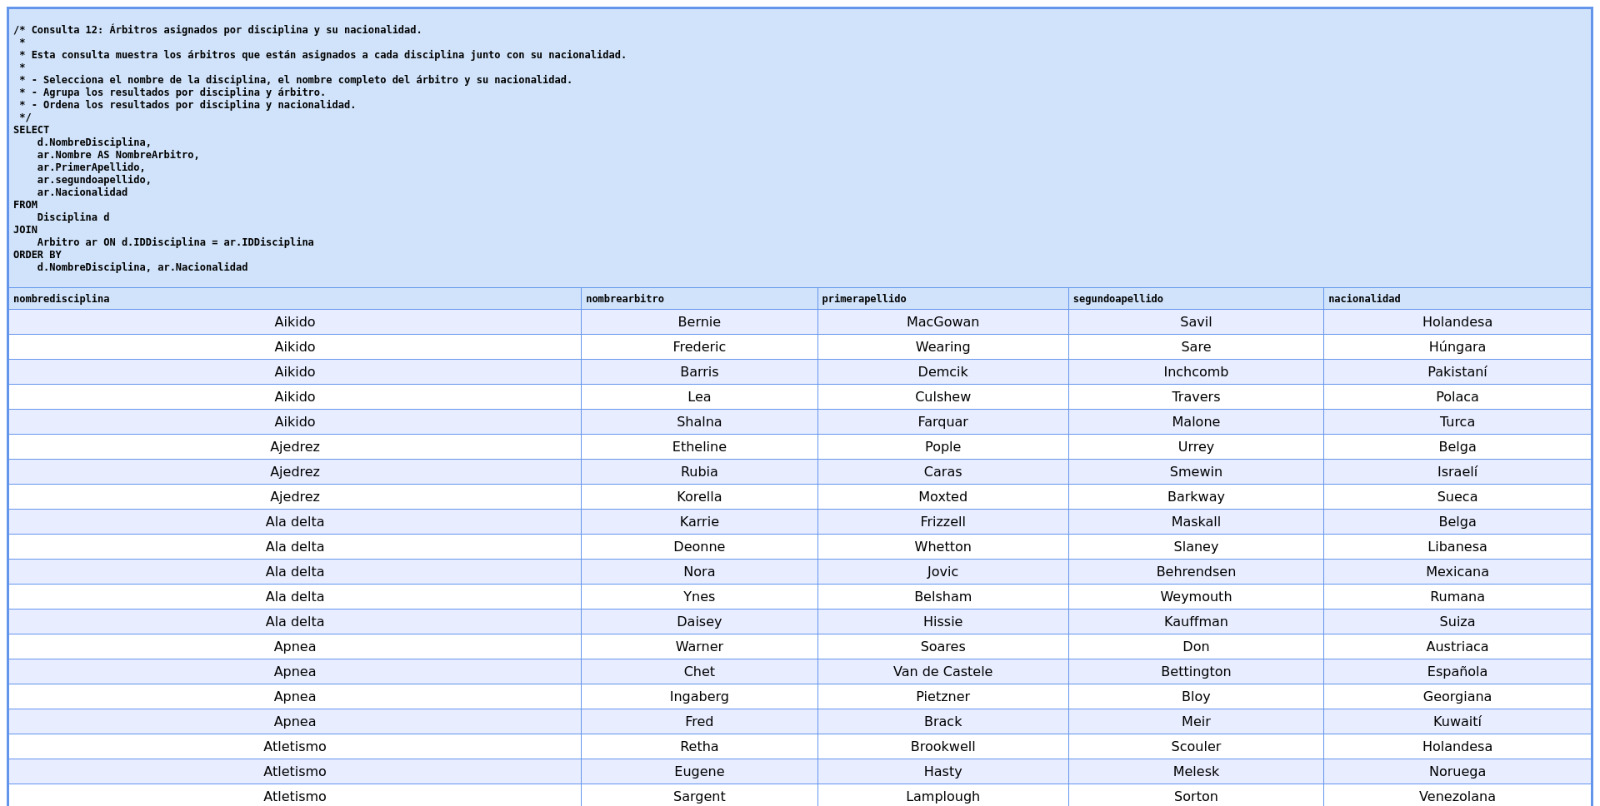
\includegraphics[width=16.5cm]{resources/Consulta12.jpeg} 
    
   Consulta 12. Árbitros asignados por disciplina y su nacionalidad.
\end{center}

\textbf{Propósito de la consulta}

El objetivo de esta consulta es obtener una lista de los árbitros asignados a cada disciplina, incluyendo su nacionalidad. Esto permite analizar la distribución de los árbitros entre las disciplinas y verificar la diversidad cultural representada en el equipo de árbitros.

\textbf{Desglose de la consulta}

\begin{itemize}
   \item \textbf{Selección de columnas (\texttt{SELECT})}:
   \begin{itemize}
       \item \texttt{d.NombreDisciplina}: Nombre de la disciplina deportiva.
       \item \texttt{ar.Nombre}: Nombre del árbitro.
       \item \texttt{ar.PrimerApellido} y \texttt{ar.SegundoApellido}: Apellidos del árbitro.
       \item \texttt{ar.Nacionalidad}: Nacionalidad del árbitro.
   \end{itemize}

   \item \textbf{Tablas involucradas (\texttt{FROM} y \texttt{JOIN})}:
   \begin{itemize}
       \item \texttt{Disciplina (d)}: Contiene información sobre las disciplinas deportivas.
       \item \texttt{Arbitro (ar)}: Contiene información sobre los árbitros.
       \item Se realiza un \texttt{JOIN} entre ambas tablas usando la relación \texttt{d.IDDisciplina = ar.IDDisciplina}, lo que asocia cada árbitro con su respectiva disciplina.
   \end{itemize}

   \item \textbf{Ordenamiento de resultados (\texttt{ORDER BY})}:
   \begin{itemize}
       \item Los resultados se ordenan primero por \texttt{d.NombreDisciplina} (nombre de la disciplina) y luego por \texttt{ar.Nacionalidad} (nacionalidad del árbitro).
   \end{itemize}
\end{itemize}

\textbf{Análisis detallado}

\begin{enumerate}
   \item \textbf{Relación entre tablas:}
   \begin{itemize}
       \item Existe una relación directa entre las tablas \texttt{Disciplina} y \texttt{Arbitro} a través de la clave foránea \texttt{ar.IDDisciplina}, que apunta a \texttt{d.IDDisciplina}.
       \item Esto implica que cada árbitro está asignado a una única disciplina.
   \end{itemize}
   
   \item \textbf{Uso de columnas seleccionadas:}
   \begin{itemize}
       \item Se seleccionan tanto datos descriptivos de las disciplinas como la información personal y de nacionalidad de los árbitros, para proporcionar un contexto completo de las asignaciones.
   \end{itemize}
   
   \item \textbf{Ordenamiento:}
   \begin{itemize}
       \item El ordenamiento jerárquico (por disciplina y nacionalidad) facilita la visualización de los árbitros por disciplina y permite detectar rápidamente patrones o diversidad nacional en cada deporte.
   \end{itemize}
\end{enumerate}

\textbf{Consideraciones}

\begin{itemize}
   \item \textbf{Árbitros sin asignación:}
   \begin{itemize}
       \item La consulta no incluye árbitros que no estén asignados a una disciplina, debido a la naturaleza del \texttt{JOIN}.
   \end{itemize}
   \item \textbf{Empates en la nacionalidad:}
   \begin{itemize}
       \item Si varios árbitros de la misma disciplina comparten nacionalidad, el orden entre ellos no está definido. Se puede agregar un criterio adicional en el \texttt{ORDER BY}, como el nombre completo del árbitro.
   \end{itemize}
\end{itemize}

\textbf{Utilidad de la consulta}

Esta consulta es útil para:
\begin{itemize}
    \item Monitorear la asignación de árbitros por disciplina y garantizar una distribución equitativa de recursos humanos.
    \item Identificar posibles carencias o exceso de árbitros en una disciplina específica.
    \item Analizar la diversidad nacional de los árbitros, lo que puede ser un indicador importante en eventos deportivos internacionales.
    \item Facilitar la planeación logística y la gestión de recursos para competencias futuras.
\end{itemize}